\begin{spacing}{1.3}

    \section{Introduction}

    Let's first define(informally) what is a {\bf Greedy Algorithm}. Consider for a problem 
    that requires us to find some kinds of {\it optimal solutions}, and to find it, 
    we always makes the choice that {\it looks best at current moment}, and choose it as 
    a part of our final solution.

    This idea may sound natural, simple, and even runs efficiently. Indeed it is, however, 
    one may alert that this strategy doesn't always give us the optimal solution 
    {\it of the whole problem}(we only make optimal choice at each step, we cannot guarantee 
    the solution is still optimal after all steps). We will see some problems that greedy 
    algorithm fails to find optimal.

    As you can see, greedy algorithm is really easy, while the hardest part is how to formally
    {\it prove} it. You must convince other people that your greedy algorithm is able to 
    find {\it global optimal solution} by simply grab {\it optimal solution at each step}.
    We will cover three different kinds of problems(except for Huffman Coding, which is a special one) 
    where greedy algorithm performs well, and the first two have similar proof of correctness,
    while the third one has a totally different proof.
    (You may be required to redo the proof or adapt the proof to another similar 
    problem in homework/exam)


    \section{Interval Scheduling}

    {\bf Problem:} Given $n$ jobs, where job $j$ starts at time $s_j$ and finishes at $f_j$.
    We say two jobs $i$ and $j$ are {\it compatible} or {\it not overlap} if their time intervals 
    $(s_i, f_i)\cap (s_j, f_j) = \emptyset$. Our goal is to find the maximum-size subset
    of {\it mutually compatible} jobs.
    \begin{center}
        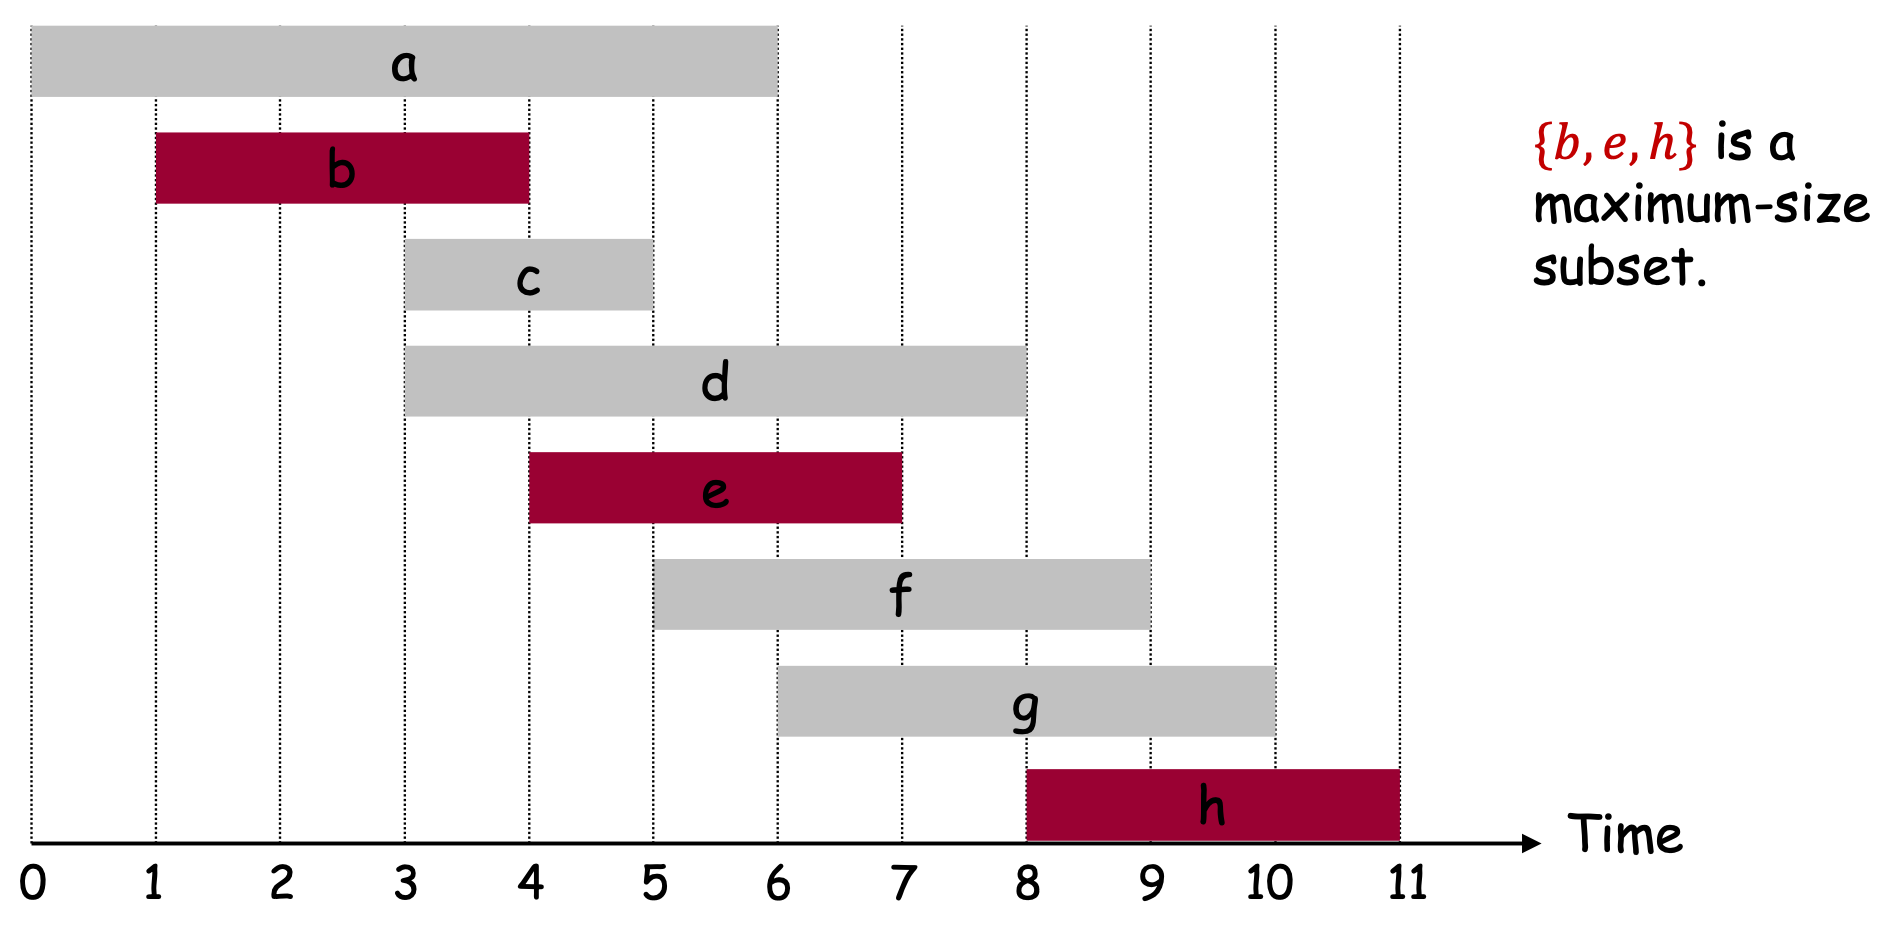
\includegraphics[scale=0.35]{images/07-interval-example.png}
    \end{center}
    In the example above, $\{b,e,h\}$ is a maximum-size subset, since you cannot find 
    a subset of size more than 4 and the jobs in that subset are mutually compatible.

    We consider to solve this problem by greedy, that is, given some jobs, we need 
    to make the best choice at current timestamp, that could make the size of subset maximized.
    So how can we maximized it? Consider choosing a job if it is compatible with all previous ones 
    that we've already taken, and not choosing it otherwise. In this way we achieve what we said that 
    ``make the best current choice''.

    However, you may easily find a counterexample, like if we first encounter a job that overlap 
    with all other jobs, then we can choose at most one job using the strategy above. So to ensure 
    its correctness, we need to first {\it consider jobs in some order}, and then use the above method.

    This order can be hard to decide, and one may think of sort jobs by:
    \begin{enumerate}
        \item increasing order of {\it start time} $s_j$,
        \item increasing order of {\it interval length} $f_j-s_j$,
        \item increasing order of {\it fewest conflicts} of each job,
        \item increasing order of {\it finish time} $f_j$.
    \end{enumerate}

    Unfortunately, we can find(not difficult) counterexamples for first three orders:
    \begin{center}
        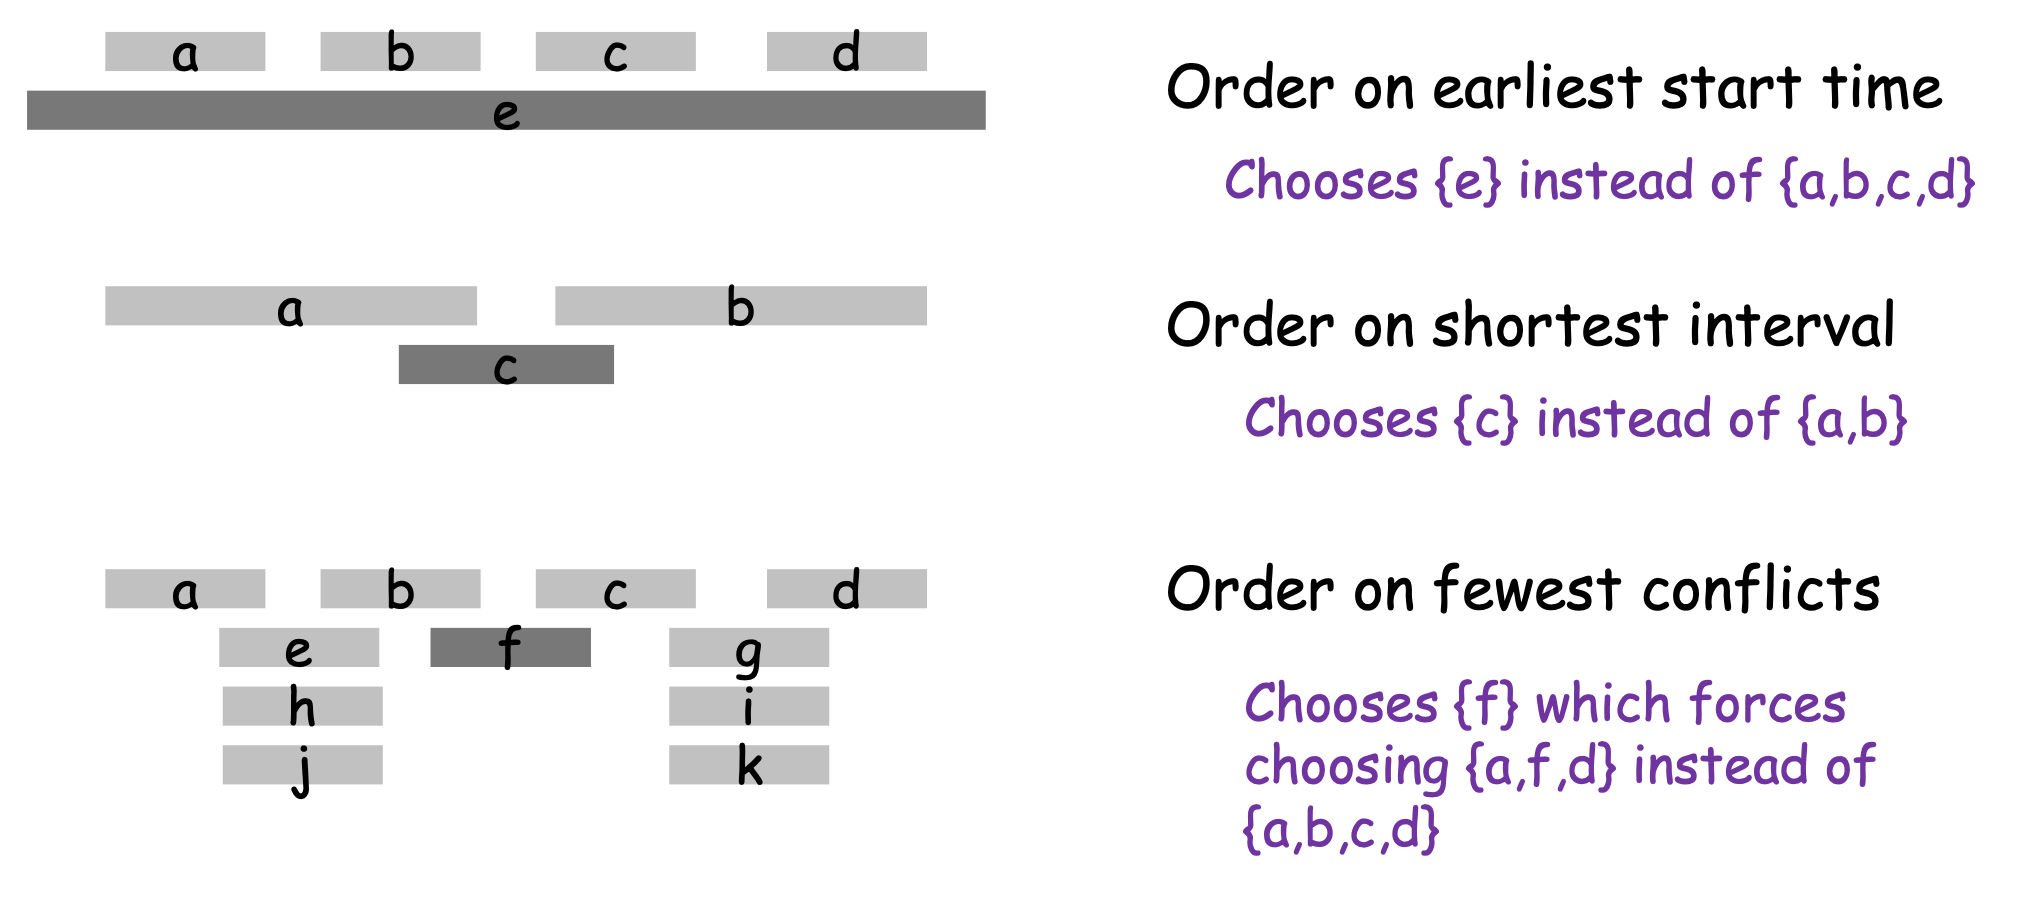
\includegraphics[scale=0.35]{images/07-interval-countereg.png}
    \end{center}

    The fourth order, i.e., sort jobs by {\it finish time}, can actually guarantee the greedy 
    algorithm to be optimal. This is not easy to find out, but the intuition is that 
    we can leave {\it maximum time} for scheduling {\it the rest of jobs}.

    You may want to review this image:
    \begin{center}
        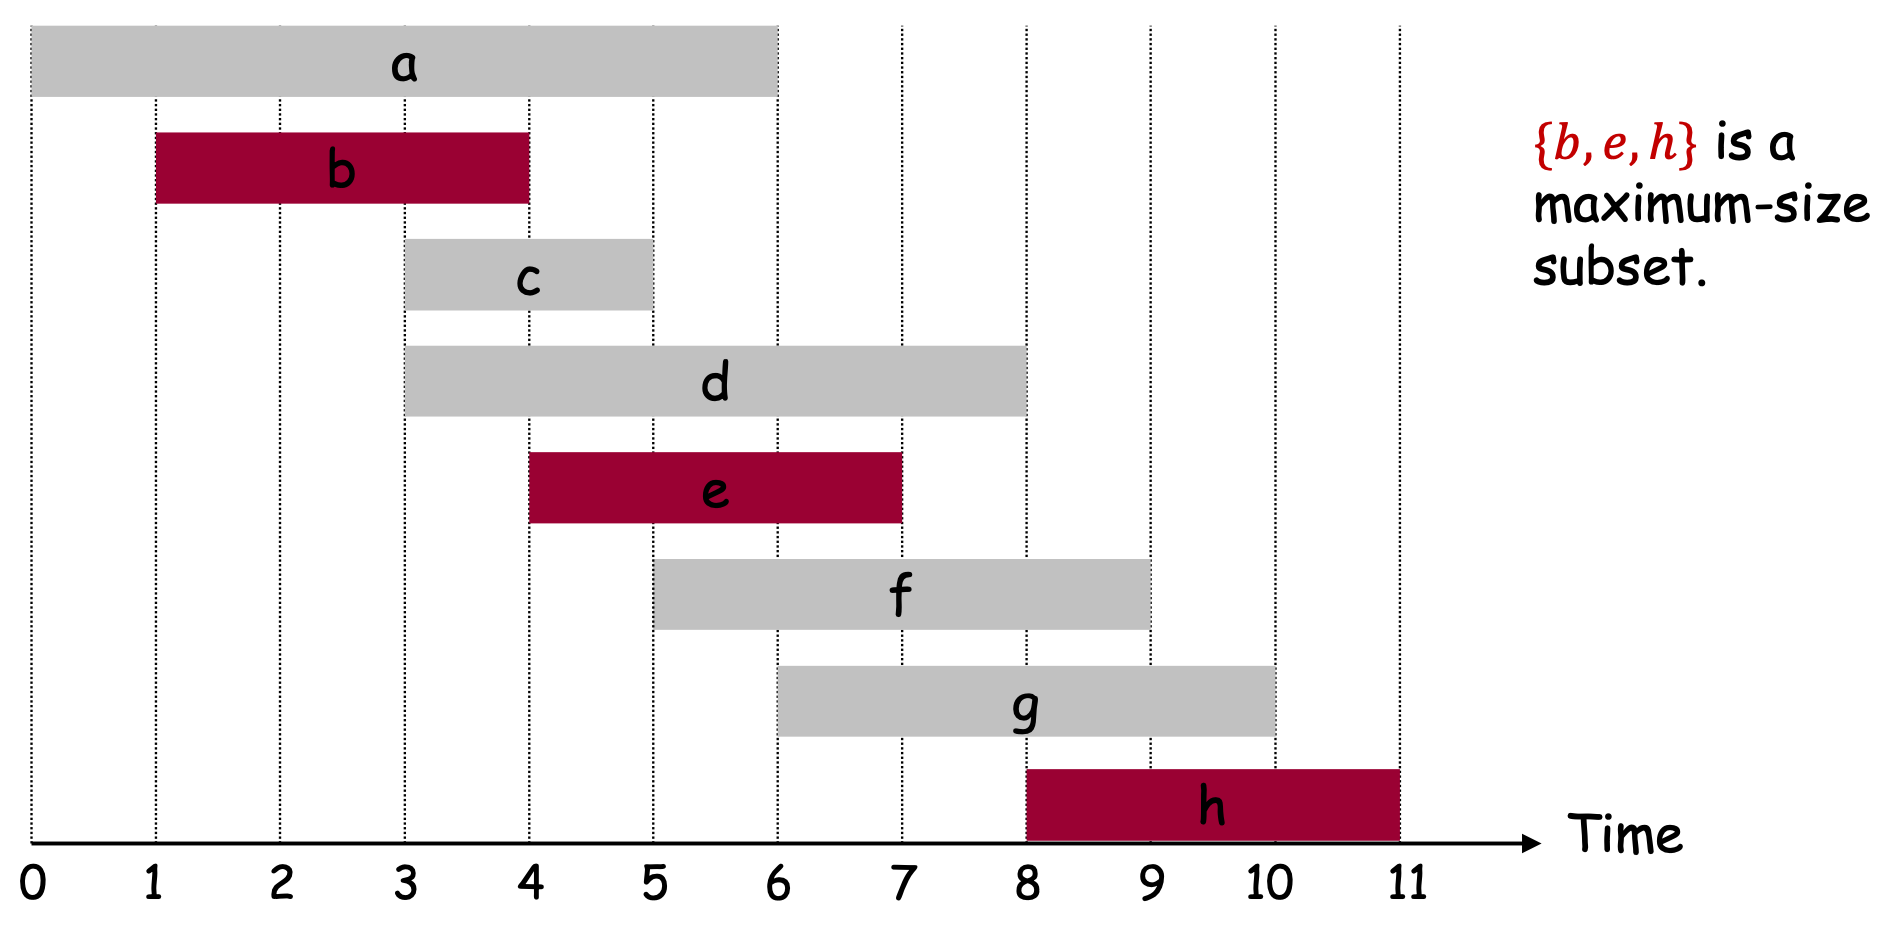
\includegraphics[scale=0.35]{images/07-interval-example.png}
    \end{center}
    We first give the code that implements this algorithm, and then formally prove it.
    
    \begin{algorithm*}
        \caption{Interval-Schedule($(s_1,f_1), \cdots, (s_n, f_n)$)}
        Sort jobs by finish time so that $f_1\le f_2\le \cdots \le f_n$

        $A\lar \emptyset$ \qquad \tcp{$A$ is the set to store the subset we found}

        $last \lar 0$   \qquad \tcp{$last$ records the {\it finish time} of last job we've chosen}

        \For{$j\lar 1$ to $n$}{
            \tcp{If job $j$ is compatiable with previous jobs, i.e., starts no earliear than 
            the finish time of last job we've chosen}
            \If{$s_j\ge last$}{
                $A\lar A\cup \{j\}$\qquad \tcp{Add job $j$ into our set}

                $last \lar f_j$ \qquad \tcp{Update $last$}
            }
        }
        return $A$
    \end{algorithm*}

    The running time of this algorithm is dominated by sorting process, which causes $\Theta(n\log n)$.

    Now let's prove the correctness of this algorithm, i.e., {\it the greedy algorithm is optimal}.

    Assume the set of jobs we get from greedy algorithm is different from an optimal set.
    Let $i_1,i_2,\cdots, i_k$ be the set of jobs found by greedy algorithm, while 
    $j_1,j_2,\cdots,j_m$ be the set of jobs in optimal solution. Our basic idea is to 
    {\it modify} optimal solution into the same as our greedy solution, while at the same time 
    {\it ensure the solution is still optimal after modification.}

    We start by finding largest possible value of $r$ such that $i_1=j_1, i_2=j_2, \cdots, i_r=j_r$,
    that is, find the last job that are the same in both sets. Thus, $i_{r+1}\ne j_{r+1}$.

    Notice in our greedy algorithm, we sort jobs by increasing of finish time, so if $i_{r+1}\ne j_{r+1}$,
    there must be job $i_{r+1}$ finishes no later than $j_{r+1}$, i.e., $f_{i_{r+1}}\le f_{j_{r+1}}$.
    \begin{center}
        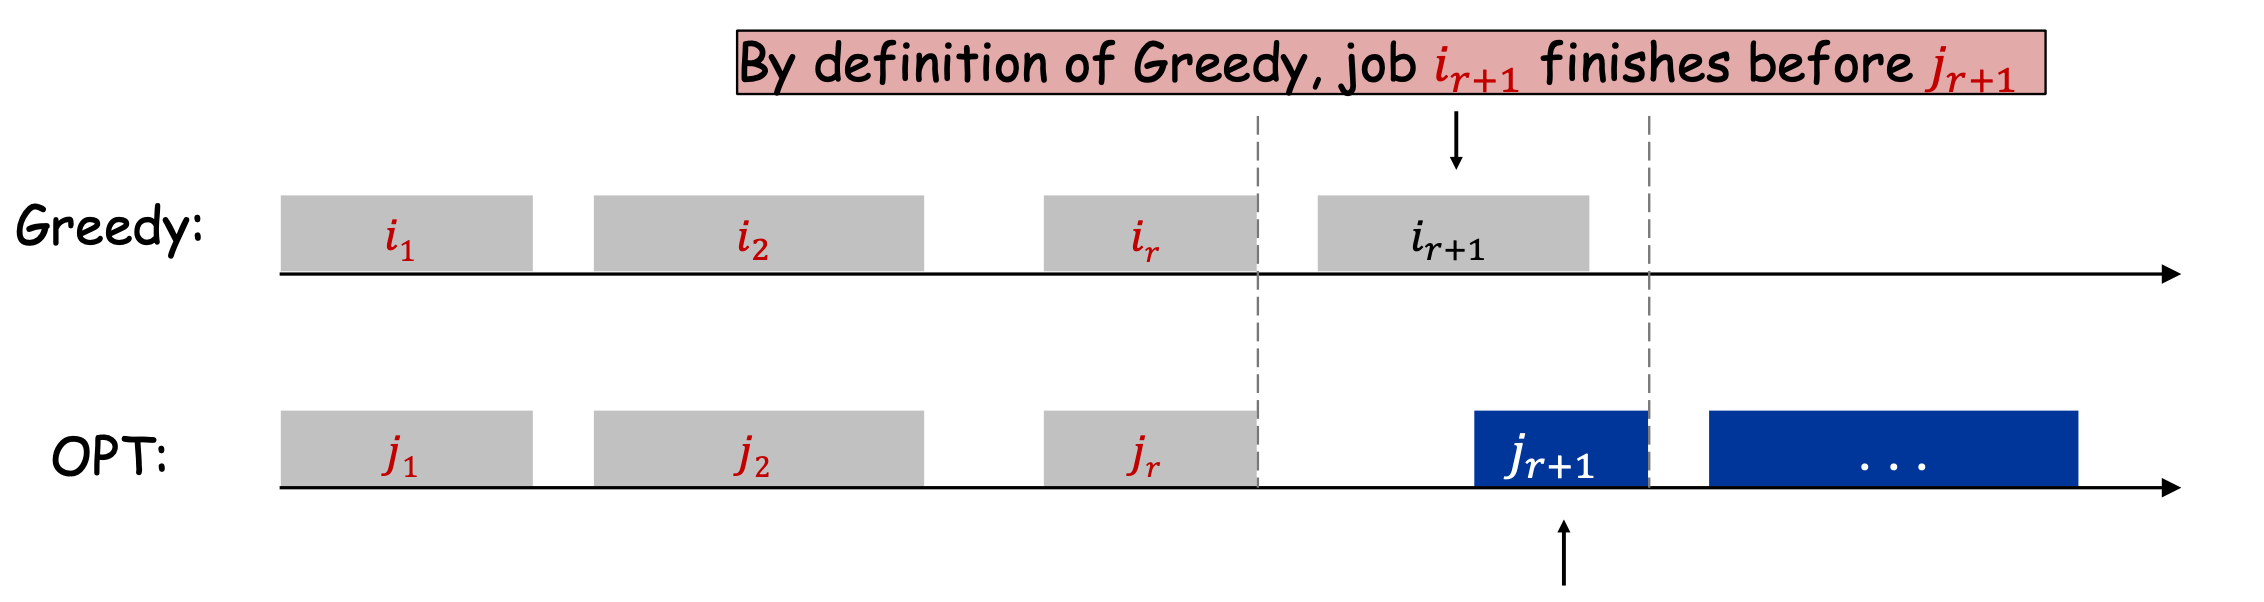
\includegraphics[scale=0.35]{images/07-interval-proof.png}
    \end{center}
    Then, we try to modify optimal solution, say, create $OPT^\star$ from $OPT$ by just replacing 
    $j_{r+1}$ with $i_{r+1}$. Notice now $OPT^\star$ is still a legal solution, the jobs are
    still mutually compatible, and $OPT^\star$ has the same size as $OPT$, so $OPT^\star$ is 
    also an optimal solution!

    Let's do this process again, until the optimal solution is the same as greedy.
    A minor problem is that they may not have the same size, i.e., $k\ne m$. 
    If this happens, the only possible is $k<m$, since $m$ is the size of optimal solution, 
    it must be the largest! However, $k<m$ is also impossible, since after replacing 
    all jobs using above method, $i_1=j_1, i_2=j_2,\cdots, i_k=j_k$. If there is 
    still jobs in optimal solution, say $j_{k+1}$, that is compatible with all previous 
    jobs, then our greedy algorithm must would have chosen that(this holds immediately 
    from our algorithm). So there must be $k=m$.


    \vspace{0.5in}
    \section{Knapsack}

    {\bf Problem:} Given $n$ items, where item $i$ has weight $w_i$ and value $v_i$.
    You now only has a knapsack that can holds weight at most $W$, you want to fill 
    your knapsack with as much {\it value} as possible. Notice in this problem an item 
    can be {\it partially used}, like each item is some liquid.

    The idea is quite simple: since we can partially use an item, we just first choose 
    items with largest ``value-weight ratio'', i.e., largest $\dfrac{v_i}{w_i}$.
    If the bag is full, we stop choosing, otherwise, we repeat the process 
    on remaining items.

    \begin{algorithm*}
        \caption{Fractional-Knapsack($w_1, v_1, w_2, v_2, \cdots, w_n, v_n, W$)}
        Sort items so that $\dfrac{v_1}{w_1}\ge \dfrac{v_2}{w_2}\ge \cdots \ge \dfrac{v_n}{w_n}$

        $w\lar W$\qquad \tcp{$w$ records how many {\it more} weight can the knapsack hold}

        \For{$i\lar 1$ to $n$}{
            \tcp{If $w_i\le w$, we can choose whole item, otherwise, we can only choose partial}
            \eIf{$w_i\le w$}{
                $x_i\lar 1$\qquad \tcp{$x_i$ records how much of the item is chosen, 1 means whole}

                $w\lar w-w_i$\qquad \tcp{update remaining capacity of the knapsack}
            }{
                $x_i\lar w/w_i$\qquad \tcp{choose partial}

                return \qquad \tcp{No need to update $w$, since we are already done}
            }
        }
        return
    \end{algorithm*}

    Again, its running time depends on the sorting process, which is $\Theta(n\log n)$.

    To prove the correctness of this greedy algorithm, we can assume $\disp \sum_{i=1}^n w_i\ge W$, 
    i.e., the knapsack is fully packed. Otherwise, the algorithm just takes all items thus 
    is trivially optimal.

    For the following proof, we assume the items are already {\it sorted by 
    } ``value-weight ratio''.
    
    We will use the technique in last example, let the greedy solution be 
    $G=(x_1,x_2,\cdots, x_k, 0, \cdots, 0)$, where for $i<k, x_i=1$, since we fully take those items,
    and for $k$-th item, $0\le x_k\le 1$, since we may or may not fully take it, and 
    for $i>k, x_i=0$, since they are not so ``valuable'' and we didn't take it.
    Also consider some optimal solution $OPT=(y_1,y_2,\cdots, y_n)$. Note that since 
    both of them must fully pack the knapsack, there must be:
    $$\sum_{i=1}^k x_i w_i=\sum_{i=1}^n y_i w_i = W$$

    Again, we find the first item $i$ where $G$ and $OPT$ differ:
    
    \begin{tabular}{ccccccccccccc}
        $G$ & $=$ & $x_1$ & $x_2$ & $x_3$ & $\cdots$ & $x_{i-1}$ & {\blue $x_i$} & $\cdots$ & $x_k$ & $\cdots$ & 0 & 0\\
        $OPT$ & $=$ & $x_1$ & $x_2$ & $x_3$ & $\cdots$ & $x_{i-1}$ & {\blue $y_i$} & $\cdots$ & $y_k$ & $\cdots$ & $y_{n-1}$ & $y_n$\\
    \end{tabular}
   
    Since our algorithm is greedy, it will take item $i$ as much as possible, 
    so there must be $x_i>y_i$. We let $\Delta x=x_i-y_i>0$.

    We can then modify the $OPT$ as follows:
    \begin{itemize}
        \item change $y_i$ to $x_i$, i.e., take as much as what we've taken in greedy 
        \item remove some items in $i+1,\cdots,n$, such that their total weights equal 
        to $\Delta x$.
        \item What we have done up to now is that we take more item $i$ while 
        throw away equal weights of $i+1,\cdots,n$ items.
        \item Since those items are sorted by ``value-weight ratio'', as stated before, 
        the value of $OPT$ after modification {\it must have not decreased}.(think why)
        \item Since the value of $OPT$ must have already been the largest before modification, 
        so the value of $OPT$ must not change. 
        \item So the new solution $OPT^\star$ must still be an optimal solution.
    \end{itemize}

    In the same way, we repeat this process, and will eventually convert $OPT$ to $G$.

    Hence our greedy algorithm yields an optimal solution, the correctness is proved.

    \vspace{0.3in}
    One thing worths mentioning is that if this problem is modified into ``items 
    cannot be partially used'', i.e., you can only either choose the item, or 
    not choose the item(also known as ``0/1 Knapsack Problem''), then there is no 
    greedy algorithm that yields optimal solution. We will come back to this in 
    Dynamic Programming.


    \section{Interval Partitioning}

    {\bf Problem:} There are $n$ lectures, where lecture $j$ starts at 
    time $s_j$ and finishes at time $f_j$. Our goal is to find the {\it minimum 
    number of classrooms} to schedule ALL lectures so that no two occurs at the 
    same time in the same room.

    For example, the below schedule, which uses 3 classrooms, is the optimal 
    solution for given lectures.
    \begin{center}
        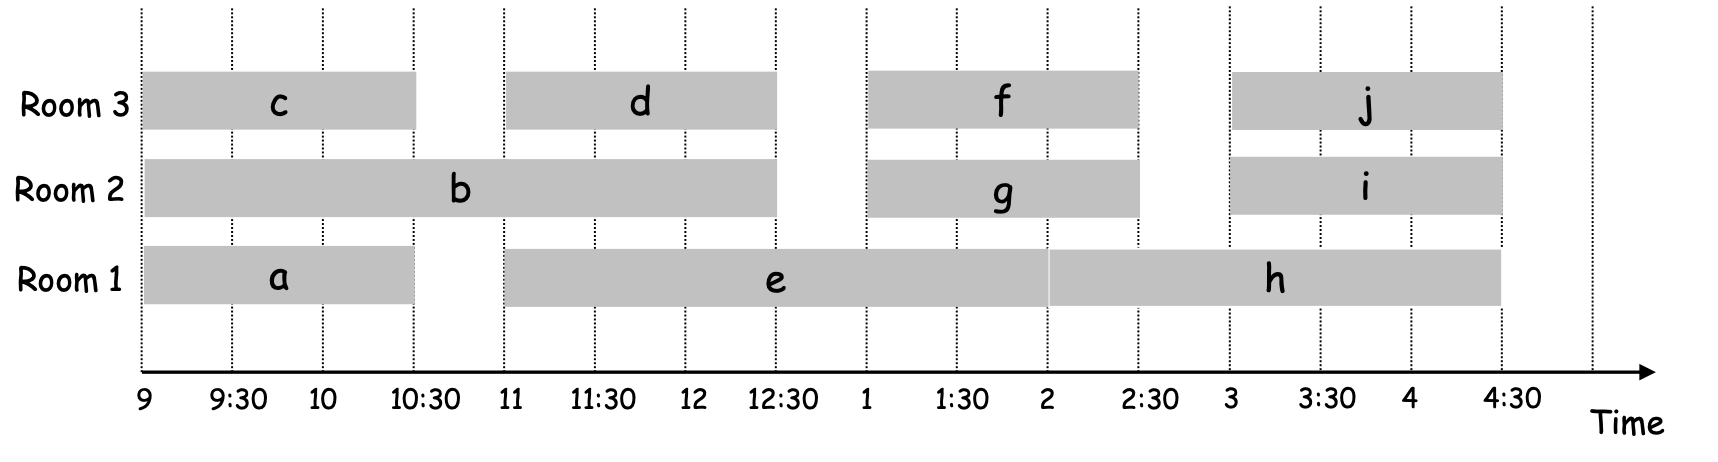
\includegraphics[scale=0.5]{images/07-interval-part-demo.png}
    \end{center}

    For this problem, we sort lectures in increasing order of {\it start time}, 
    and assign each lecture to any compatible classroom. That is, 
    for each lecture $j$, if there is an existing classroom $k$ such that 
    $k$ is empty during time interval $(s_j, f_j)$, then we assign lecture $j$
    to classroom $k$.

    Otherwise, if all existing classrooms are incompatible with the lecture, 
    we allocate it to a new classroom.

    The algorithm is shown below:

    \begin{algorithm*}[htbp]
        \caption{Interval-Partition($(s_1,f_1)\cdots (s_n, f_n)$)}
        Sort intervals by starting time so that $s_1\le s_2\le \cdots \le s_n$

        $d\lar 0$\quad \tcp{$d$ records \# of classrooms used so far}

        \For{$j\lar 1$ to $n$}{
            \eIf{lecture $j$ is compatible with some classroom $k$}{
                schedule lecture $j$ in classroom $k$
            }{
                allocate a new classroom numbered $d+1$

                schedule lecture $j$ in classroom $d+1$

                $d\lar d+1$
            }
        }
        return $d$
    \end{algorithm*}

    (Before we prove this is optimal, you should convince yourself that sorting by 
    finish time does not yield optimal.)

    



    \section{Huffman Coding}



    \newpage
    \section{Exercises}

    {\it Those problems are extracted from COMP3711 past paper or previous assignments. 
    Please find solution after the problems.}

    1. (2019Spring, Midterm, 3, 18pts) {\bf Interval Scheduling}
    
    In this problem you will describe and explain the correctness of the interval scheduling algorithm that was taught in class.
    
    {\it The Interval Scheduling Problem}: Suppose that you are given $n$ intervals $I_{1}, I_{2}, \ldots, I_{n-1}, I_{n}$ that are sorted from left to right according to some criterion. For $1 \leq i \leq n$, the start and finish times of $I_{i}$ are denoted by $s_{i}$ and $f_{i}$, respectively. Two intervals $I_{i}$ and $I_{j}$ are compatible if their interior do not overlap, i.e., $s_{i} \geq f_{j}$ or $s_{j} \geq f_{i}$. The interval scheduling problem is to select a subset of mutually compatible intervals that has the maximum size.
    
    {\it The Greedy Algorithm}: The following pseudocode describes a greedy algorithm for the interval scheduling problem.
    
    1. $A \leftarrow\left\{I_{1}\right\}$;\\
    2. for $j=2$ to $n$\\
    3. \quad if $I_{j}$ is compatible with the intervals in $A$\\
    4. \quad \quad \quad $A \leftarrow A \cup\left\{I_{j}\right\} ; \quad /^{*}$ add $I_{j}$ to the set $A * /$\\
    5. output the set $A$

    We have not specified HOW the intervals are sorted. Consider the following two ways of sorting:
    
    \noindent (a) By increasing starting time, i.e., $s_{1} \leq s_{2} \leq \cdots \leq s_{n}$.\\
    (b) By increasing finishing time, i.e., $f_{1} \leq f_{2} \leq \cdots \leq f_{n}$.
    
    Answer the following question separately for each of the two sorting orders in (a) and (b) above.
    
    {\bf Will the greedy algorithm return a subset of mutually compatible intervals that has the maximum size? Explain.}
    
    If the answer is yes, provide a formal proof of correctness.
    
    If the answer is no, provide a counterexample. Your counterexample should specify a set of input intervals. You should state the subset returned by the greedy algorithm and explain why that subset is not a correct solution.


    \newpage
    2. (2021Spring, Final, 3, 14pts) {\bf Greedy Classroom Scheduling}

    Recall the greedy Interval Partitioning algorithm taught in class. The input was $n$ pairs of numbers $\left(s_{i}, f_{i}\right), i=1, \ldots, n$ for which $s_{i}<f_{i}$. Each pair represented a class: $s_{i}$ is class $i$ 's starting time, $f_{i}$ is its ending time. The goal was to find the minimum number of classrooms required to schedule all lectures so that no two occur at the same time in the same room. The algorithm taught in class is given below:
    
    1) Sort intervals by starting time so that $s_{1} \leq s_{2} \leq \cdots \leq s_{n}$\\
    2) $d \leftarrow 0 \quad$ \% \# classrooms used so far\\
    3) for $j \leftarrow 1$ to $n$\\
    4) \quad if lecture $j$ is compatible with some classroom $k$ then $\left(^{*}\right)$\\
    5) \quad \qquad schedule lecture $j$ in classroom $k\left(^{* *}\right)$\\
    6) \quad else\\
    7) \quad \qquad allocate a new classroom $d+1$\\
    8) \quad \qquad schedule lecture $j$ in classroom $d+1(* * *)$\\
    9) \quad \qquad $d \leftarrow d+1$
    
    (a) Prove that this algorithm gives the correct answer, i.e., it only opens the minimum number of classrooms necessary to schedule all classes.
    
    (b) Explain how to implement this algorithm in $O(n \log n)$ time. You need to say
    
    \qquad (i) what data structure you are using, and, in particular,

    \qquad (ii) how you use it to implement lines $4,5,8$ and

    \qquad (iii) why your algorithm requires $O(n \log n)$ time.

    \newpage
    3. (2020Spring, Final, 1, 15pts) {\bf Greedy Algorithms}

    Given two sequences of characters $X=\left(x_{1}, \ldots, x_{m}\right)$ and $Y=\left(y_{1}, \ldots, y_{n}\right)$ with $m \leq n$, design an $O(n)$ time algorithm that determines if $X$ is a subsequence of $Y$.
    
    Formally, $X$ is a subsequence of $Y$

    \qquad if there exists $1 \leq j_{1}<j_{2}<\cdots<j_{m} \leq n$ such that $x_{i}=y_{j_{i}}$.
    
    Example: let $Y=A B B C B D A B, X_{1}=B C B A$ and $X_{2}=B D B A$.
    
    Then $X_{1}$ IS a subsequence of $Y$, but $X_{2}$ is NOT a subsequence of $Y$.
    
    Your algorithm should return "YES" if $X$ is a subsequence of $Y$ and "NO" if $X$ is not a subsequence of $Y$.
    
    You can assume that your inputs are given as two character arrays $X[1 \ldots m]$ and $Y[1 \ldots n]$ storing $X$ and $Y$.
    
    (A) Using documented psuedocode, clearly describe how your algorithm works.
    
    (B) Formally prove that your algorithm is correct
    
    (C) Explain why it runs in $O(n)$ time.
    
    In part (B), put every argument on a separate line with space betwen the lines.
    
    Write your proof clearly. If you use induction in your proof, you must clearly state what your induction hypothesis is. If you prove by contradiction, clearly identify the statement that is being assumed wrong, etc.


    \newpage
    4. (2019Spring, Midterm, 2, 10pts) {\bf Huffman Coding}

    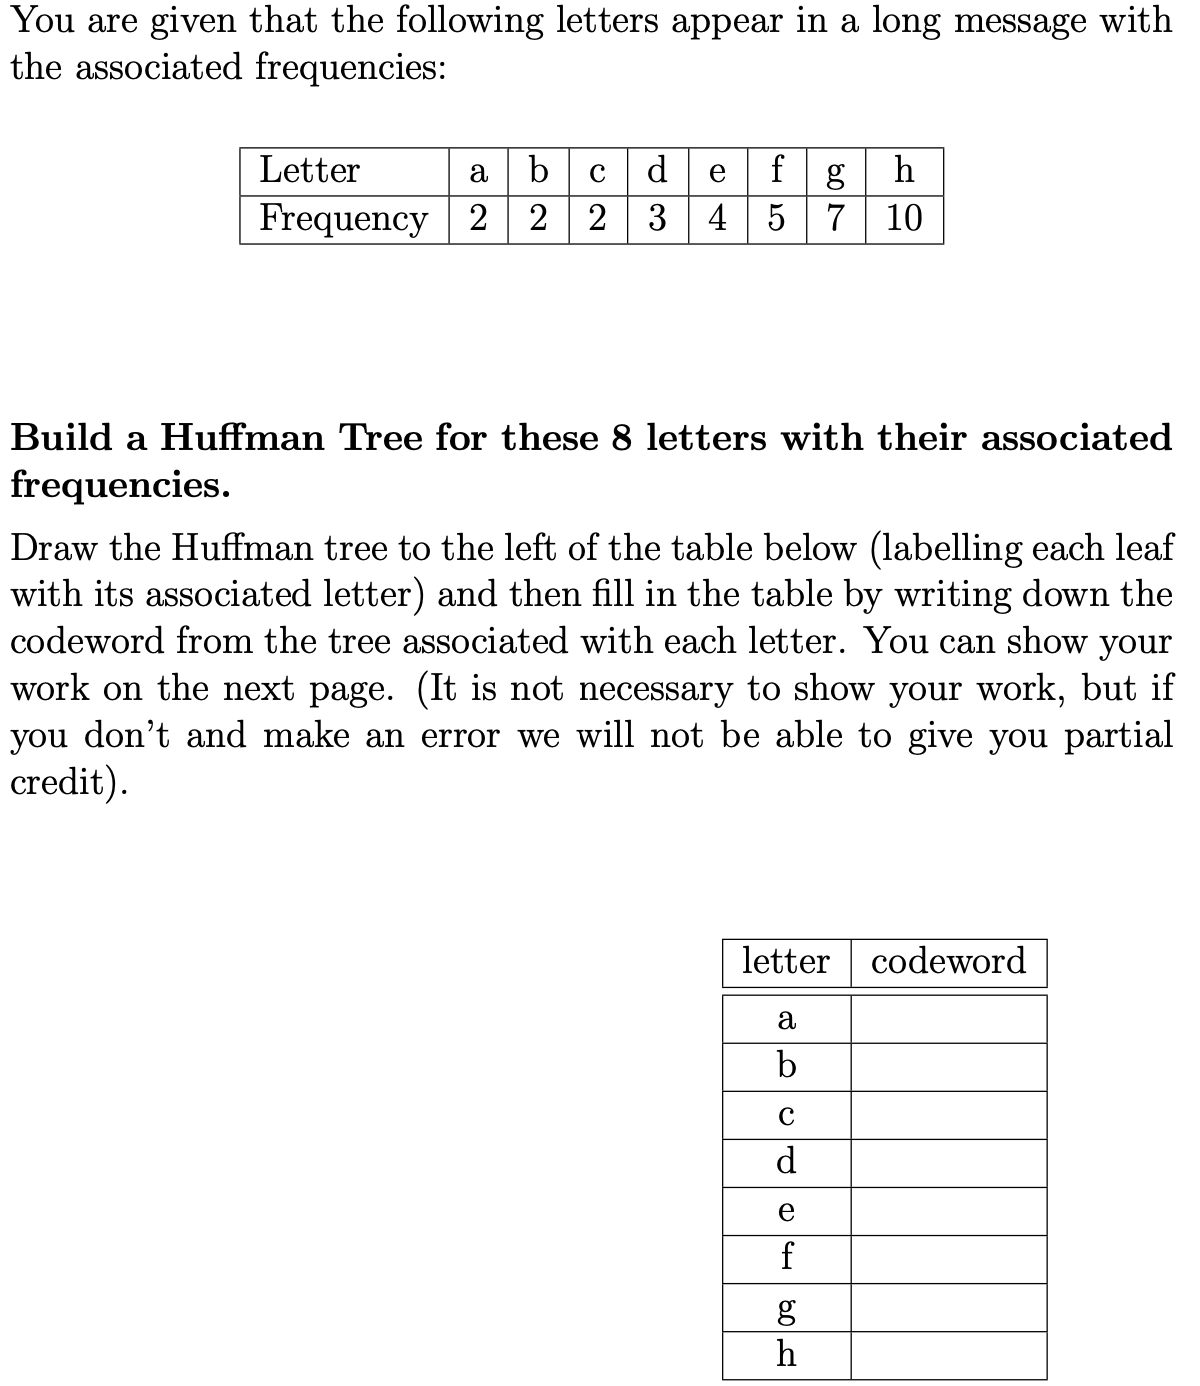
\includegraphics[scale=0.65]{images/07-exercise-2019s-huffman-question.png}

    \newpage
    5. (2021Fall, Assignment 3, Problem 4, 29pts) {\bf Greedy Covering}

    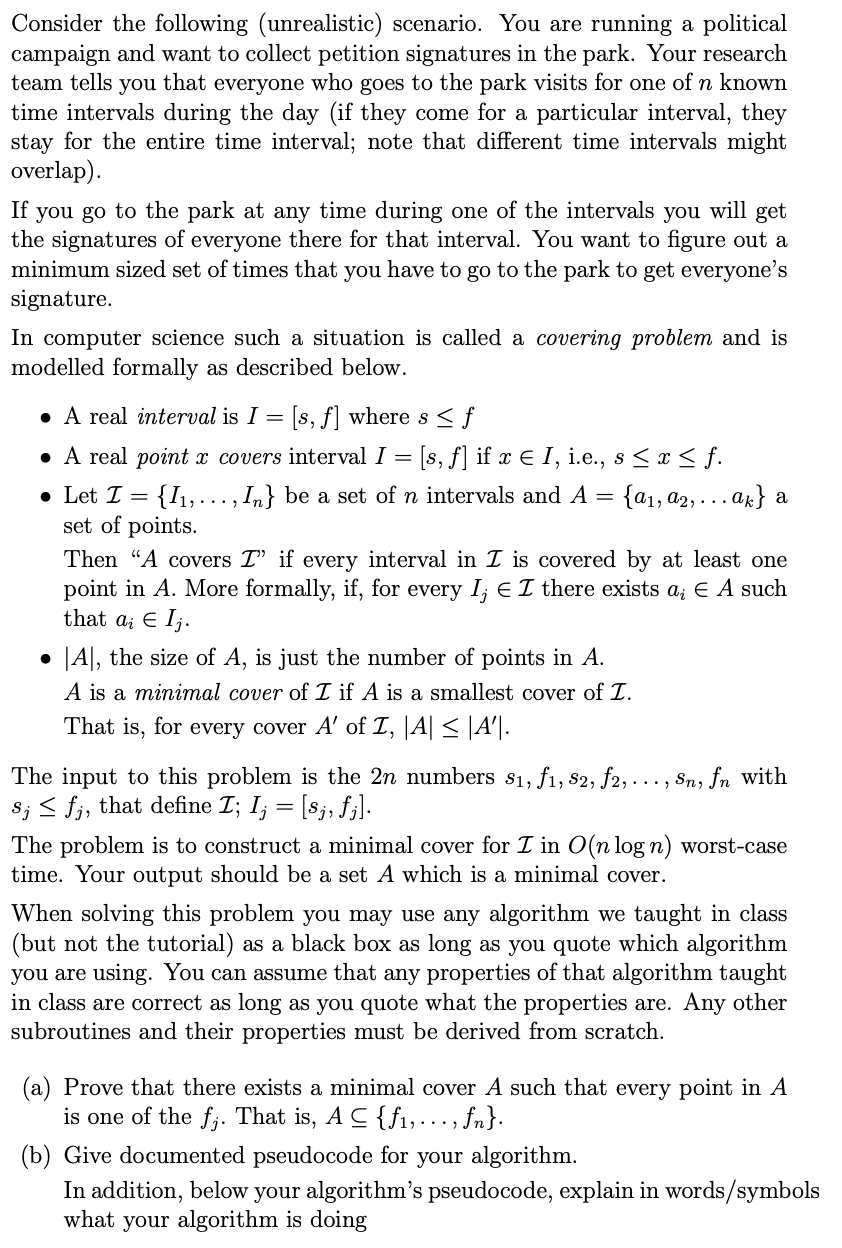
\includegraphics[scale=1.05]{images/07-exercise-2021f-hw-question.png}

    \newpage
    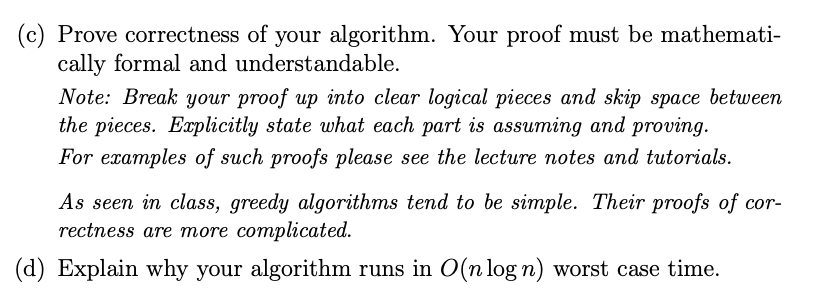
\includegraphics[scale=1.05]{images/07-exercise-2021f-hw-question2.png}



    \newpage
    \section{Solution to Exercises}

    1. (2019Spring, Midterm, 3, 18pts) {\bf Interval Scheduling} 

    (a) When the intervals are sorted by increasing start time the solution does not have to be correct. Consider this counterexample:
    $$
    I_{1}=(1,6), I_{2}=(2,3), I_{3}=(4,5).
    $$
    The optimal solution is $\left\{I_{2}, I_{3}\right\}$ while the greedy algorithm will return just the one interval $\left\{I_{1}\right\}$.
    
    (b) When the intervals are sorted by increasing finish time the solution us optimal.
    
    This is the analysis from the class notes:
    
    \setlength{\parindent}{2em}

    (a) Assume greedy is different than OPT
    
    (b) Let $i_{1}, i_{2}, \ldots, i_{k}$ denote the set of intervals selected by greedy We are ordering them so that $i_{1}<i_{2}<\cdots$
    
    (c) Let $j_{1}, j_{2}, \ldots, j_{m}$ denote the set of intervals selected by OPT Again we are ordering them so that $j_{1}<j_{2}<\cdots$
    Since an interval must end before the next one starts this means $f_{j_{r}} \leq s_{j_{r+1}}$ for all $r$
    
    (d) Note that by the definition of OPT, $m \geq k$.
    
    (e) Find largest possible value of $r$ such that $i_{1}=j_{1}, i_{2}=j_{2}, \ldots$, $i_{r}=j_{r}$.
    This means that we can write OPT as
    $$
    O P T=i_{1}, i_{2}, \ldots, i_{r}, \mathbf{j}_{\mathbf{r}+1}, j_{r+2}, \ldots, j_{m} .
    $$
    Note that it's possible that $r=0$.
    
    (f) By the definition of the greedy algorithm $j_{r+1}$ can not finish before $i_{r+1}$, otherwise the greedy algorithm would have chosen $j_{r+1}$. This means that $f_{i_{r+1}} \leq f_{j_{r+1}}$
    
    (g) From the comment in (c) above, this automatically implies that $f_{i_{r+1}} \leq f_{j_{r+1}} \leq s_{j_{r+2}}$.
    This simply means that we can replace $j_{r+1}$ with $i_{r+1}$ in OPT and still have a set of compatable coverings. This gives us
    $$
    O P T^{\prime}=i_{1}, i_{2}, \ldots, i_{r}, \mathbf{i}_{\mathbf{r}+\mathbf{1}}, j_{r+2}, \ldots, j_{m} .
    $$
    Now note that size $\left(O P T^{\prime}\right)=m=\operatorname{size}(O P T)$ so $O P T^{\prime}$ is also optimal.
    
    (h) We have therefore found an optimal solution that agrees with OPT with at least $r+1$ places instead of $r$ places.
    
    (i) We can repeat lines (a)-(g) until we have found an optimal solution OPT that agrees with greedy on all of its first $k$ places
    
    (j) If $m>k$ then greedy could have chosen $j_{k+1}$ after choosing $i_{k}$. Since greedy did not choose it, $j_{k+1}$ does not exist so $m=k$.
    
    (k) Since $m=k$, greedy is optimal

    \setlength{\parindent}{0em}

    \vspace{0.5in}
    2. (2021Spring, Final, 3, 14pts) {\bf Greedy Classroom Scheduling} 

    (a) Here is the proof we derived in class.
    \begin{itemize}
        \item (A) The depth of a set of open intervals is the maximum number of classes that exist at any instant of time.
        \item  - Let $t$ be some time at which depth classes exist simultaneously. Such a $t$ must exist from the definition of depth.
        \item  - At this time $t$, at least $d$ classrooms must be open to host the depth classes.
        \item  - $\Rightarrow$ (B) any class scheduling solution must open at least depth classrooms
        \item - Now, let $d$ be the number of classrooms opened by the greedy algorithm.
        \item - Classroom $d$ is opened because we needed to schedule a lecture, say $j$, that is incompatible with all $d-1$ other classrooms.
        \item - Since we sorted by start time, all these incompatibilities are caused by lectures that all start no later than $s_{j}$ and finish later than $s_{j}$
        \item - Thus, there is a time at which $d$ lectures all overlap. The time is $s_{j}+\epsilon$ for some $\epsilon>0$; the $d$ lectures are the $d-1$ incompatible ones and lecture $j$,
        \item - $\Rightarrow(\mathrm{C})$ depth $\geq d$
        \item - Since every schedule must use at least depth classrooms and greedy uses only $d \leq$ depth classrooms, greedy uses no more than any other solution so greedy is optimal.
    \end{itemize}

    (b) We can keep the classrooms in a min-heap (min priority queue) using the finishing times of the last class in the room as the classroom's key.
    
    To check in line 4 whether there is a compatible classroom we do an extract$\min$ to find the minimum finishing time currently stored in the priority queue.
    
    If line 5 is called, then just insert the new finishing time $s_{j}$ to p.queue
    
    If line 8 is called, then re-insert that minimum finishing time back into the p.queue AND insert the new finishing time $s_{j}$ into the p.queue
    
    Note that extract-mins and inserts can be performed in $O(\log N)$ time in a min priority queue with $N$ items. Since the number of items in the queue at any specific time will be $O(n)$, each extract-min and insert operation will $\operatorname{cost} O(\log n)$ time; thus, each call to line $(*),(* *)$ or $(* * *)$ will require only $O(\log n)$ time.
    
    Since each of lines $4,5,7$ are called at most once for each value of $j$, the total work for performing them is $O(n \log n)$ time. The sort in line (1) also requires $O(n \log n)$ time so the entire algorithm uses only $O(n \log n)$ time.


    \vspace{0.5in}
    3. (2020Spring, Final, 1, 15pts) {\bf Greedy Algorithms} 

    {\it The solution to this problem is so long, please refer to past paper.}

    \vspace{0.5in}
    4. (2019Spring, Midterm, 2, 10pts) {\bf Huffman Coding}

    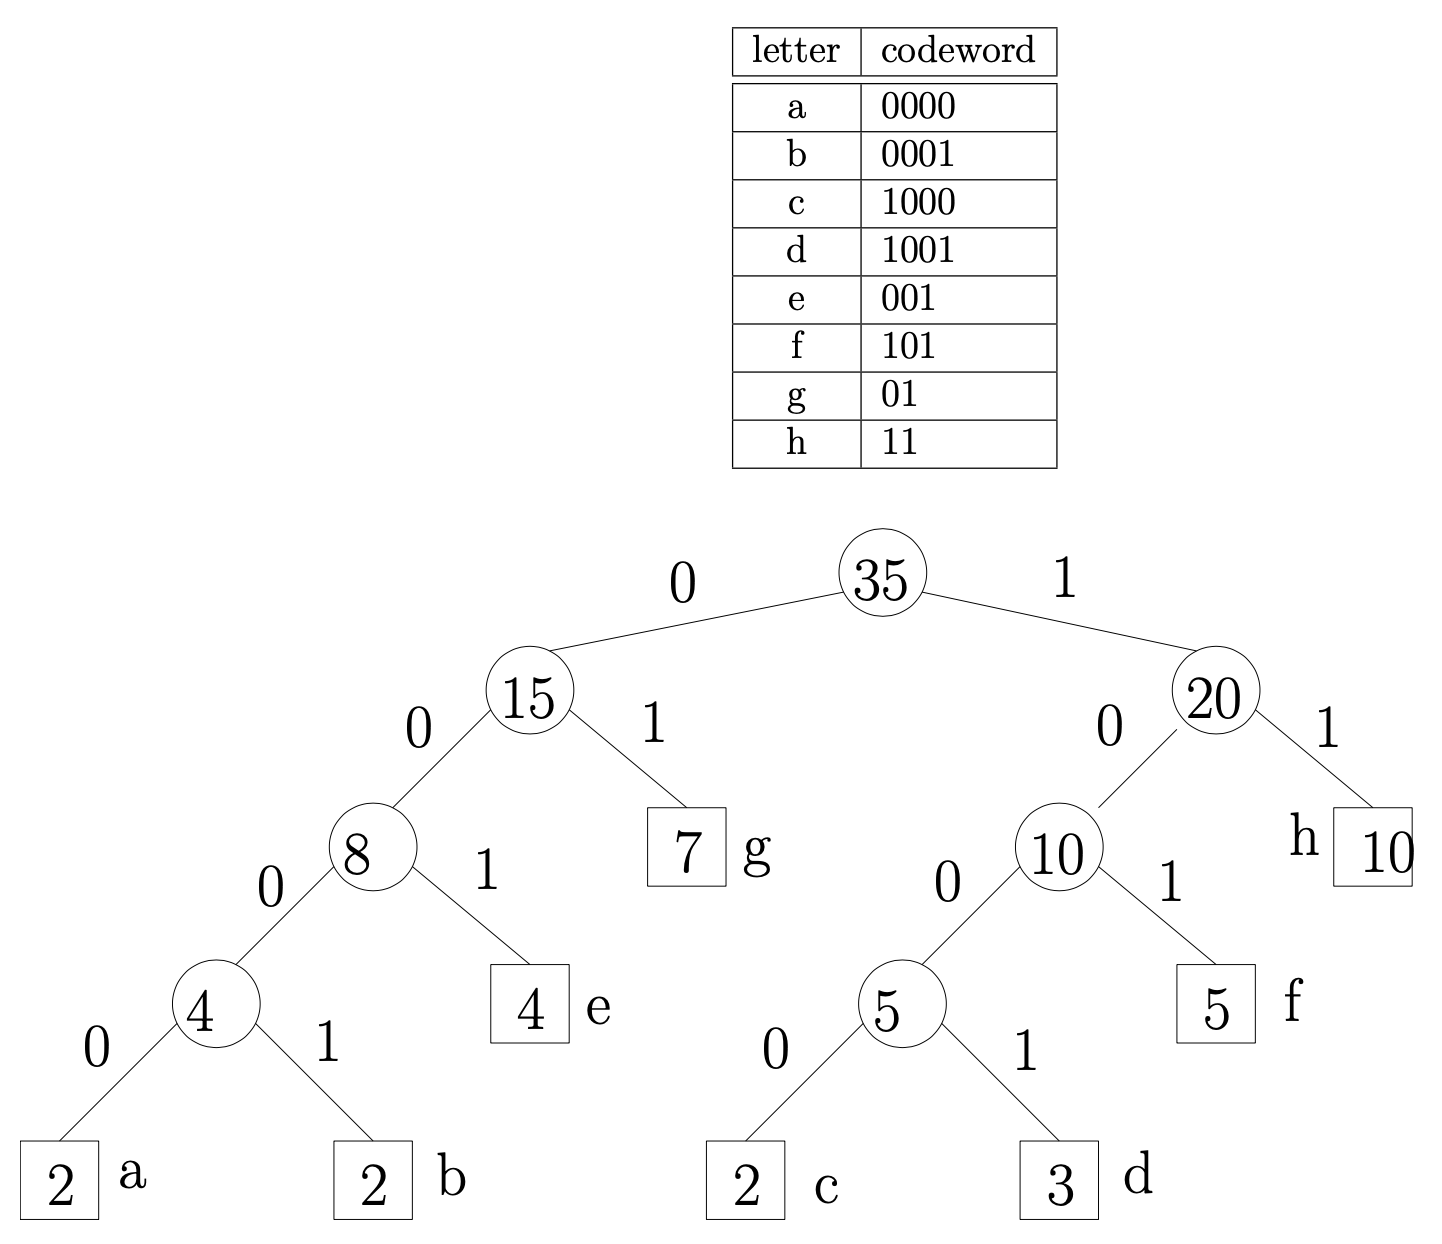
\includegraphics[scale=0.55]{images/07-exercise-2019s-huffman-sol.png}

    \newpage
    5. (2021Fall, Assignment 3, Problem 4, 29pts) {\bf Greedy Covering} 

    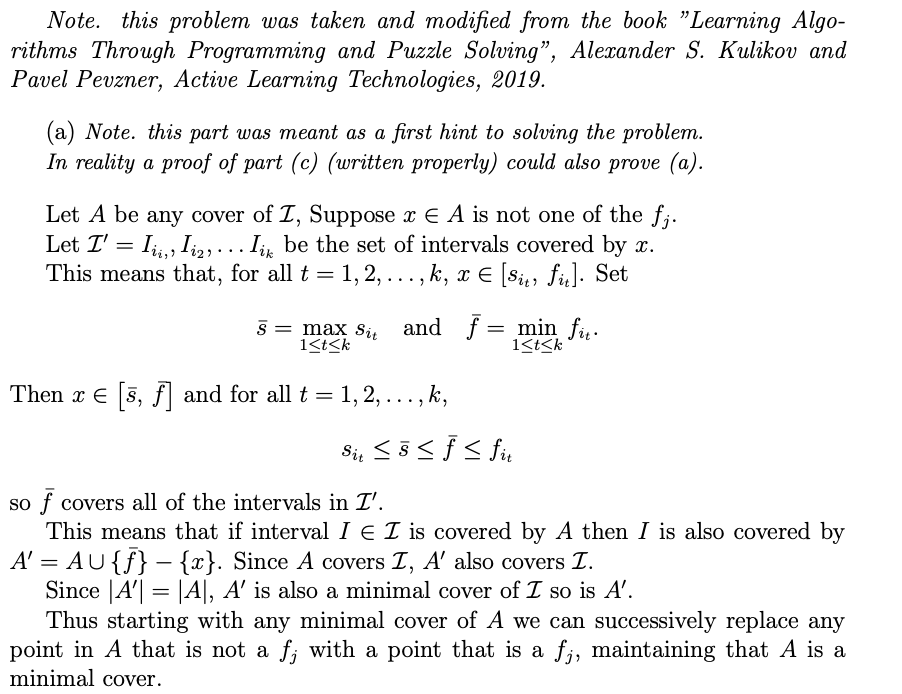
\includegraphics[scale=1.05]{images/07-exercise-2021f-hw-sol1}

    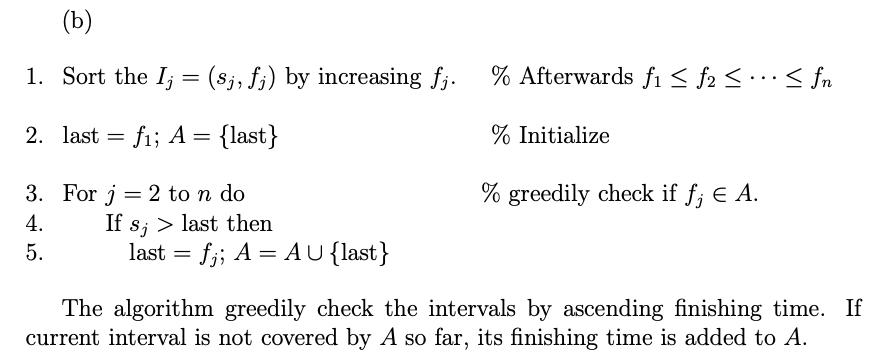
\includegraphics[scale=1.05]{images/07-exercise-2021f-hw-sol2}

    \newpage
    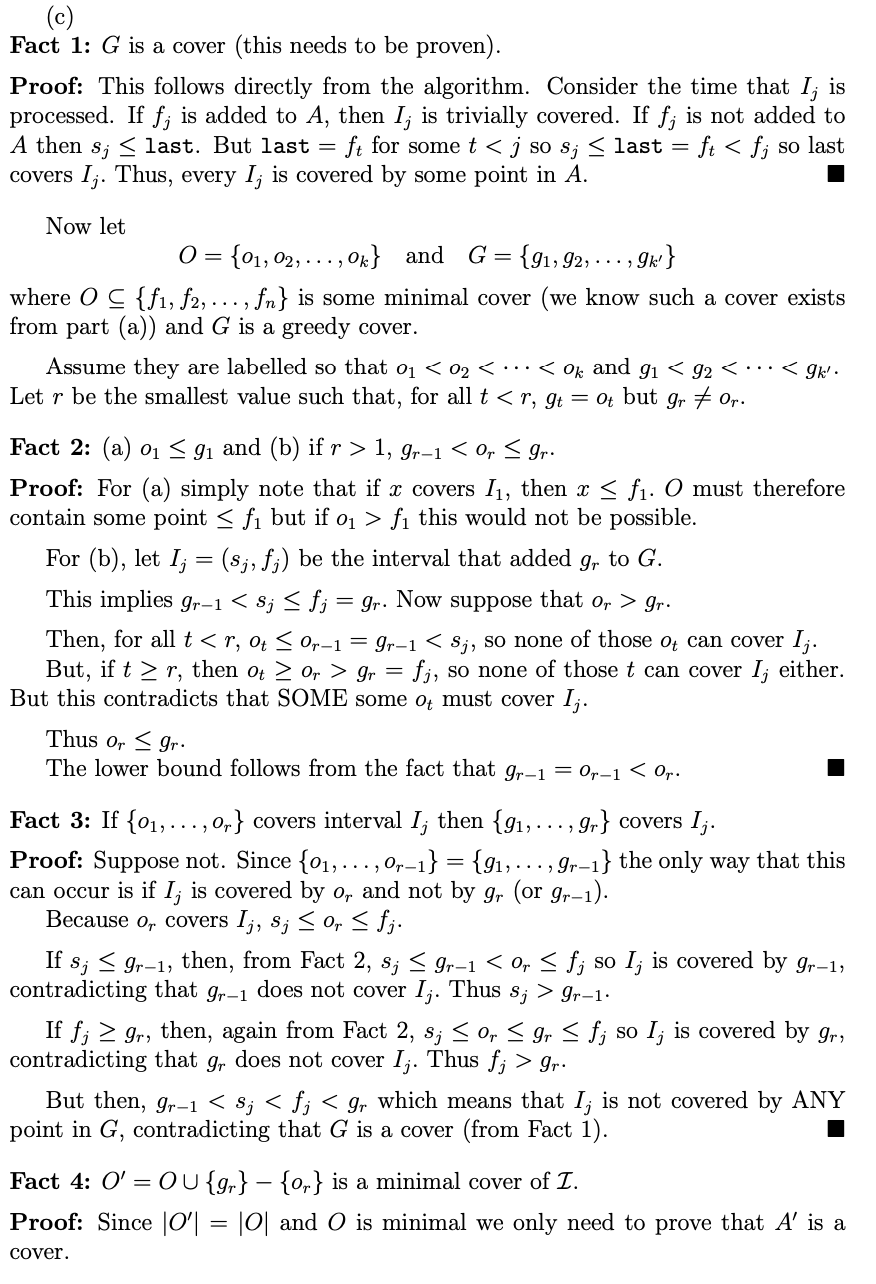
\includegraphics[scale=1.05]{images/07-exercise-2021f-hw-sol3}

    \newpage
    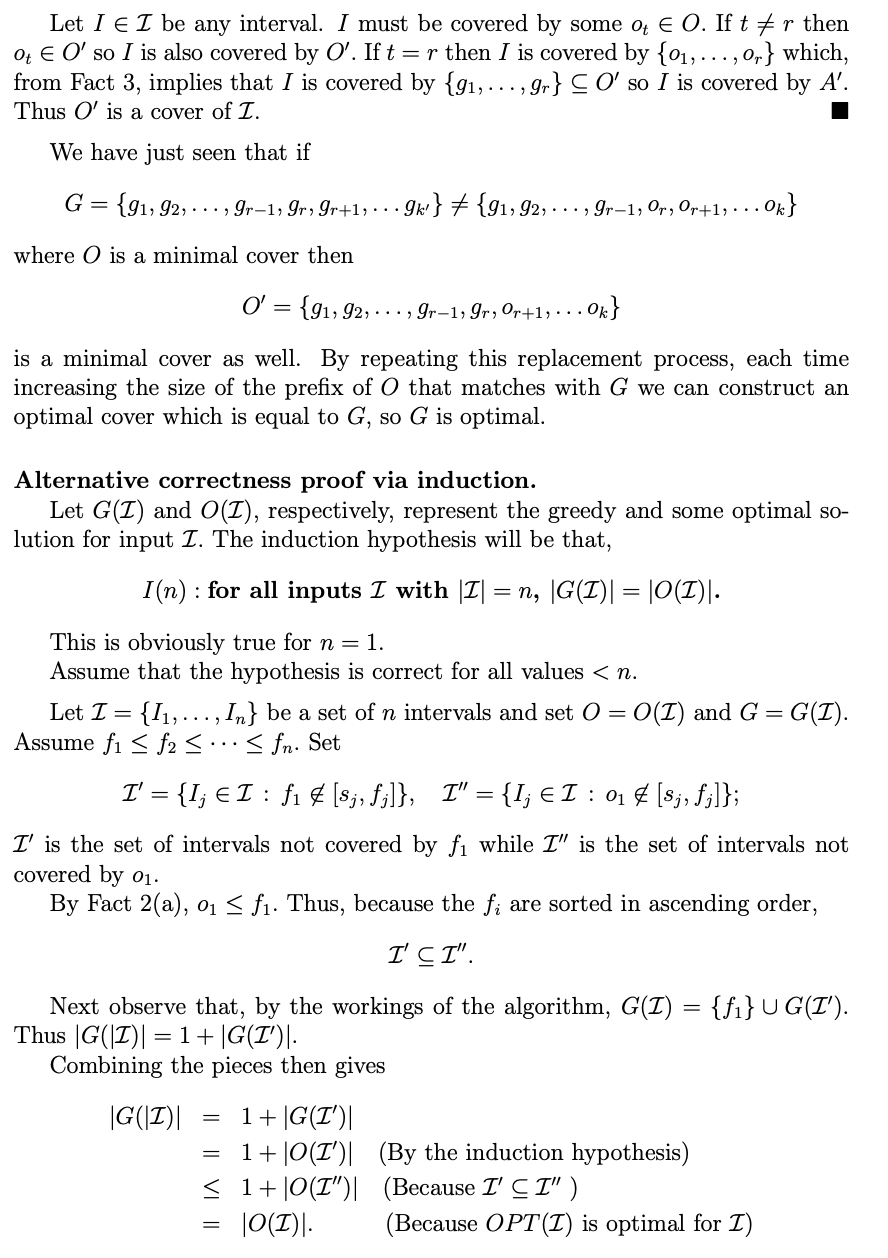
\includegraphics[scale=1.05]{images/07-exercise-2021f-hw-sol4}

    \newpage
    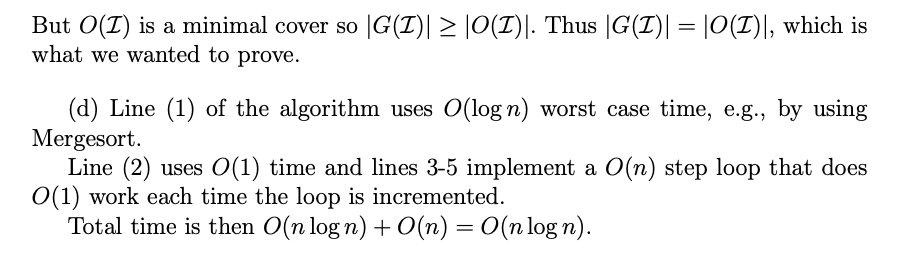
\includegraphics[scale=1.00]{images/07-exercise-2021f-hw-sol5}

\end{spacing}